% VUT FIT MITAI
% MSZ 2021/2022
% Author: Vladimir Dusek
% Login: xdusek27

%%%%%%%%%%%%%%%%%%%%%%%%%%%%%%%%%%%%%%%%%%%%%%%%%%%%%%%%%%%%%%%%%%%%%%%%%%%%%%%%

% Path to figures
\graphicspath{{tin/zasobnikove_automaty/figures}}

%%%%%%%%%%%%%%%%%%%%%%%%%%%%%%%%%%%%%%%%%%%%%%%%%%%%%%%%%%%%%%%%%%%%%%%%%%%%%%%%

\chapter{TIN~--~Zásobníkové automaty (jazyky přijímané ZA, varianty ZA).}

%%%%%%%%%%%%%%%%%%%%%%%%%%%%%%%%%%%%%%%%%%%%%%%%%%%%%%%%%%%%%%%%%%%%%%%%%%%%%%%%

\section{Zdroje}

\begin{compactitem}
    \item \path{tin_2021_merged.pdf}
    \item \path{TIN_2020-10-06.mp4}
    \item \path{TIN_2020-10-13.mp4}
\end{compactitem}

%%%%%%%%%%%%%%%%%%%%%%%%%%%%%%%%%%%%%%%%%%%%%%%%%%%%%%%%%%%%%%%%%%%%%%%%%%%%%%%%

\section{Zásobníkový automat}

Zásobníkové automaty dokáží přijímat bezkontextové jazyky.

\paragraph{Zásobníkový automat} Zásobníkový automat (ZA) je sedmice $M = (Q, \Sigma, \Gamma, \delta, q_0, Z_0, F)$, kde \begin{compactitem}
    \item $Q$ je konečná množina stavů;
    \item $\Sigma$ je vstupní abeceda;
    \item $\Gamma$ je zásobníková abeceda;
    \item $\delta$ je přechodová funkce (parciální funkce), \begin{compactitem}
        \item $\delta : Q \times \Sigma \times \Gamma \rightarrow 2^{Q \times \Gamma^*}$;
    \end{compactitem}
    \item $q_0$ je výchozí stav, \begin{compactitem}
        \item $q_0 \in Q$;
    \end{compactitem}
    \item $Z_0$ je výchozí symbol na zásobníku, \begin{compactitem}
        \item $Z_0 \in \Gamma$;
    \end{compactitem}
    \item $F$ je množina koncových stavů, \begin{compactitem}
        \item $F \subseteq Q$;
    \end{compactitem}
\end{compactitem}

\paragraph{Konfigurace ZA} Konfigurace ZA je trojice $(q, w, \alpha) \in Q \times \Sigma^* \times \Gamma^*$, kde \begin{compactitem}
    \item $q$ je aktuální stav;
    \item $w$ je nezpracovaná část vstupního řetězce;
    \item $\alpha$ je obsah zásobníku.
\end{compactitem}

\paragraph{Počáteční konfigurace ZA} Počáteční konfigurace ZA je taková konfigurace $(q, w, \alpha)$, kde $w \in \Sigma^*$ je vstupní řetězec, $q \in Q$ je výchozí stav a $\alpha = Z \in \Gamma$ je výchozí symbol na zásobníku.

\paragraph{Koncová konfigurace ZA} Koncová konfigurace ZA je taková konfigurace $(q, w, \alpha)$, kde $q \in F$, $w = \epsilon$ a $\alpha \in \Gamma^*$.

\paragraph{Přechod ZA} Přechod ZA je binární relace (značíme $\vdash$) na množině konfigurací $\vdash ~ \subseteq (Q \times \Sigma^* \times \Gamma^*)^2$, taková, že $$ (q, w, \alpha) \vdash (q', w', \alpha') \Leftrightarrow \exists a \in (\Sigma \cup \epsilon), ~ \exists Z \in \Gamma, ~ \exists \beta, \gamma \in \Gamma^* ~:~ $$

$$ ~:~ w = aw' \land \alpha = Z \beta \land \alpha' = \gamma \beta \land (q', \gamma) \in \delta(q, a, Z) $$

\begin{figure}[H]
    \centering
    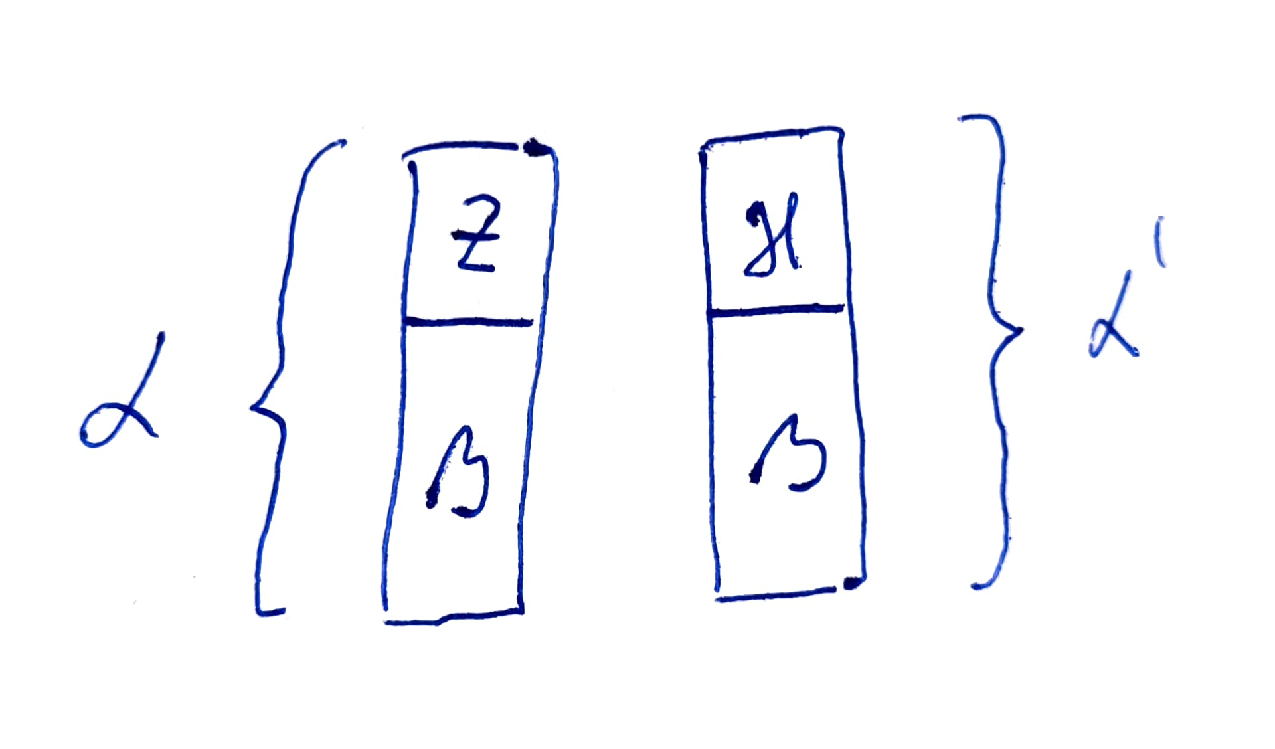
\includegraphics[width=0.35\linewidth]{za_prechod_zasobnik.pdf}
    \caption{Stav zásobníku během přechodu ZA. Platí $Z \in \Gamma,~ \alpha, \alpha', \beta, \gamma \in \Gamma^*$.}
\end{figure}

\paragraph{Jazyk přijímaný ZA} Mějme ZA $M = (Q, \Sigma, \Gamma, \delta, q_0, Z_0, F)$ a jazyk $L(M)$, který je přijímaný ZA $M$. $$ L(M) = \{ w ~|~ w \in \Sigma^* \land (q_0, w, Z_0) \vdash^* (q_f, \epsilon, \epsilon) \land q_f \in F \}$$ Avšak existují různé varianty. ZA může přijímat i v $q_f \in F$: pouze při vyprázdnění vstupu, nebo pouze při vyprázdnění zásobníku a nebo při vyprázdnění vstupu a vyprázdnění zásobníku.

%%%%%%%%%%%%%%%%%%%%%%%%%%%%%%%%%%%%%%%%%%%%%%%%%%%%%%%%%%%%%%%%%%%%%%%%%%%%%%%%

\section{Varianty zásobníkového automatu}

\paragraph{Rozšířený zásobníkový automat} \todo{todo}

\begin{figure}[H]
    \centering
    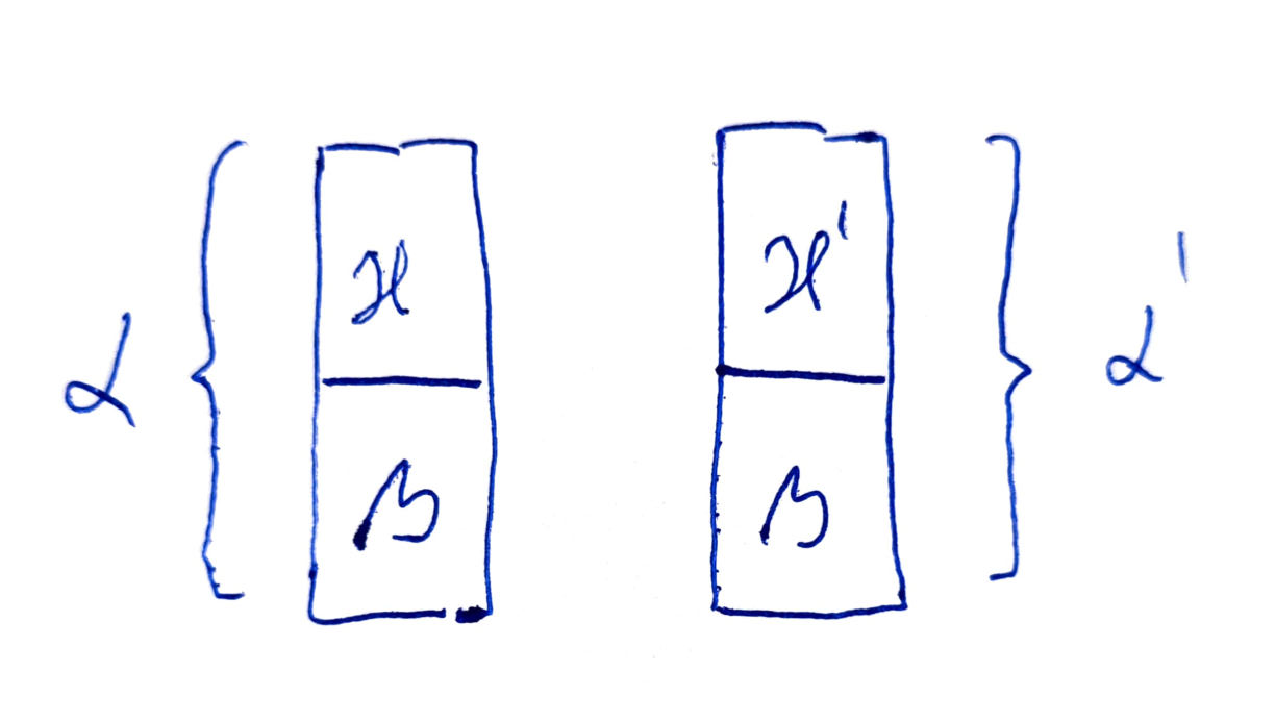
\includegraphics[width=0.35\linewidth]{rza_prechod_zasobnik.pdf}
    \caption{Stav zásobníku během přechodu RZA. Platí $\alpha, \alpha', \beta, \gamma, \gamma' \in \Gamma^*$.}
\end{figure}

\paragraph{Deterministický zásobníkový automat} \todo{todo}

\paragraph{Deterministický rozšířený zásobníkový automat} \todo{todo}
